\documentclass[12pt]{article}
\usepackage[margin=1in]{geometry}
\usepackage{natbib}
\usepackage{graphicx}
\usepackage{caption}
\usepackage{subcaption}
\usepackage{multirow}
\usepackage{longtable}
\usepackage{color}
\usepackage{hyperref}
\bibliographystyle{apalike}
\newcommand{\beginsupplement}{%
        \setcounter{table}{0}
        \renewcommand{\thetable}{S\arabic{table}}%
        \setcounter{figure}{0}
        \renewcommand{\thefigure}{S\arabic{figure}}%
     }


\begin{document}

\title{Evolutionary genomics of peach \\and almond domestication}

\author{\small\sfbf{Dianne Velasco$^{\S}$, Mallikarjuna Aradhya$^{\dag}$, Jeffrey Ross-Ibarra$^{\S\ddag}$}\thanks{Corresponding author: Department of Plant Sciences, University of California, Davis, California 95616, USA. E-mail: \mbox{rossibarra@ucdavis.edu}} \\[0.3cm]
     \small\sf $^{\S}$Department of Plant Sciences, University of California, Davis, California 95616, USA,\\
     \small\sf $^{\dag}$USDA-ARS National Clonal Germplasm Repository, Davis, California 95616, USA,\\
     \small\sf $^{\ddag}$Center for Population Biology and Genome Center, University of California, Davis, California 95616, USA}

\date{\today}
\maketitle

\section*{Introduction}
%BACKGROUND ON SPECIES
%
With approximately four hundred species, including multiple domesticated crop species, \emph{Prunus} is the largest genus in the family Rosaceae.
%reference to number of approximate number of species, number depends on reference
%
Almond, apricot, cherry, peach, and plum are the crop types found in three of the five \emph{Prunus} subgenera, subgenus \emph{Amygdalus} has the most morphologically distinct crops, sibling species \emph{P. persica} (Mill.) D. A. Webb (peach) and \emph{P. dulcis} (L.) Batsch (almond).
%
Domestication of almond and peach occurred approximately 5000 years ago in the Fertile Crescent and China \citep{zohary2012domestication}, respectively, followed by global dissemination \citep{hedrick1917peaches, edwards1975almond, gradziel2011origin, zheng2014archaeological}.
%
Additionally, while \emph{Prunus} species are generally outcrossing due to gametophytic self-incompatibility with self-compatibility alleles known to exist in multiple species, peach is the only fully self-compatible diploid species in the genus. 
%
Both domestication and mating system have been shown to significantly impact genome evolution in annual species \citep{glemin2006impact, doebley2006molecular, slotte2013capsella}. 
%
However, the impacts of domestication and mating system on the genome evolution in tree species remains poorly understood \citep{mckey2010evolutionary, miller2011forest}.
\\
\\
% DOMESTICATION & PROGENITOR IDENTIFICATION
Peach and almond have similar lengths of domestication, early fruit development, perenniality, precocity, genome organization \citep{arus2012peach}, and genome size \citep{arumuganathan1991nuclear, dickson1992nuclear, baird1994estimating, loureiro2007two}.
%
The most striking differences are mature fruit morphology and mating systems, but almond and peach also generally differ in life span (longer v. shorter), chilling requirements (lower v. higher) and adventitious root generation (poor v. good).
%
The few obvious traits associated with almond domestication are reduced toxicity, thinner endocarp, and increased seed size, while domestication in peach is characterized by diverse fruit morphology (size, color, texture, shape, etc.) and self-compatibility.
%
However, traits not typically associated with domestication but common to both, such as precocity, or solely with peach, such as relative ease of adventitious rooting, may have also been targeted or incidentally selected during domestication. 
%
Unfortunately, efforts to identify wild progenitors of almond and peach \citep{verde2013high, aradhya2004molecular, zeinalabedini2010origin, mowrey1990isozyme, browicz1996genus, ladizinsky1999origin, bassi20081} by examining species relationships within the subgenus \emph{Amygdalus} have had mixed results. 
%
Given the uncertainty in identifying wild progenitors of almond and peach, domestication studies using crossing experiments are not suitable and are generally impractical in perennial crops.
%crossing experiment citation, perhaps one of Doebley's papers or others using domesticated x wild cross to identify domestication locus/loci (maize, tomato, etc.)
%
With the recent cost reductions in high throughput sequencing, using genomic resequencing is a practical approach to gain insights into domestication of perennial crops and its genome-wide nature also enables distinguishing between mating system and domestication effects.
%
\\
\\
%DOMESTICATION VERSUS SI/SC IN GENOME
In closely related species pairs with alternate mating systems, such as \emph{Arabidopsis thaliana} and \emph{A. lyrata} and \emph{Capsella rubella} and \emph{C. grandiflora} \citep{slotte2013capsella} mating system is shown to significantly affect genome evolution, such as nucleotide diversity, linkage disequilibrium (LD), heterozygosity, genome size, repeat content, and genetic load.
%
Expectation for the perennial species pair of peach (\emph{P. persica}) and almond (\emph{P. dulcis}) is that self-compatible peach has a lower genome-wide diversity than self-incompatible almond.
%
However, domestication also reduces genomic diversity, but in localized regions important to domestication \citep{glemin2006impact, doebley2006molecular, slotte2013capsella}.
%
Peach and almond have also undergone domestication, but the expectation is that localized reductions in genomic diversity are due to domestication while overall differences are due to alternate mating systems \citep{glemin2006impact, charlesworth2001breeding}. 
%
%Domestication in plants is associated with changes in many traits, such as increased size and morphological diversity of the harvested organ (seed, fruit, leaves, etc.), reduced seed dispersal, adaptation to disturbed environments, reduced toxicity, selfing, photoperiod insensitivity, etc. \citep{doebley2006molecular}, but a relative few of these changes are striking in almond or peach. 
%seed size in almond, fruit size & color in peach
%range of bloom/maturity dates for peach
%sweet kernels in almond
%what about other tree crops? (Review Miller & Gross paper)
%
\\
\\
%STUDY PURPOSE AND SUMMARY
%
Like all species within the subgenus \emph{Amygdalus}, peach and almond are both diploid, , and genetic mapping from an almond x peach $F_2$ population suggests they have a similar genomic structure \citep{dirlewanger2004comparative}. 
%
At an estimated 230 Megabases (Mb) spanning eight chromosomes, the recently sequenced peach genome \citep{verde2013high} is less than double the genome size of model plant \emph{Arabidopsis thaliana} while at 300 Mb the cytologically estimated almond genome size of almond is similar to pre-sequencing estimates of peach \citep{arumuganathan1991nuclear}. 
% efficient species
%
%Peach already serves as a model system for \emph{Prunus} and other tree crops due to its small genome (230 Mb), short generation time (2-3 years), and self-compatibility \citep{arus2012peach}.
%
%Small genome sizes, chromosome numbers, and relatively short juvenility, peach and almond support their use as a model to investigate the effects of domestication and mating system in trees.
%
Recent analysis of resequenced peach genomes indicates low genetic diversity and higher LD across the genome compared to wild peach species \citep{verde2013high}, but the few resequenced almond genomes have not been similarly assessed. 
%
%This is not unexpected considering the primary peach genetic map is based on an almond x peach $F_2$ population due to poor resolution in peach $F_2$ genetic maps \citep{arus2012peach, joobeur1998construction, aranzana2003set, dirlewanger2004comparative, dominguez2003plant}.
%
%However, due to self-incompatibility almond is expected to have higher levels of heterozygosity and lower LD compared to peach.
%
Understanding the impact of mating system on almond and peach evolutionary genomics expands the basic understanding of genome evolution in a perennial species pair with alternate mating systems. 
%is this a first for perennial species?
%
Identification of candidate domestication loci will provide an opportunity to determine which loci in almond and peach were under selection, if any are in common and whether they have similar haplotypes, and to identify similarities or differences when compared to annual crops. 
%
%Knowledge gained from these analyses provides valuable information regarding domestication loci and haplotypes, an important resource for tree breeding programs.
%
%Understanding the contributions of domestication and mating systems to genome evolution in almond and peach expands the understanding of these processes beyond annual species. 
%
Public resequenced peach genomes and almond genomes resequenced in this study provide the raw material for an evolutionary genomics investigation into the patterns of domestication and mating system in closely related perennial crop species and provide a model for evolution and domestication in tree species.
%
\\
\section*{Materials and Methods}
%
\subsection*{Samples}
Resequenced genomes of domesticated species \emph{P. dulcis} and \emph{P. persica}, fourteen and thirty-two respectively, and one each of closely related species, \emph{P. fenzliana} and \emph{P. ferganensis}, and plum outgroup, \emph{P. cerasifera} were used for analysis.
%
Of the fourteen resequenced \emph{P. dulcis} genomes, five were from public sources (four from \citealt{koepke2013comparative}(?) via NCBI SRA and one RosBREED) and nine were newly resequenced samples (one at BGI and eight at UC Berkeley).
%
Thirty-one of thirty-two \emph{P. persica} resequenced samples were from public sources (ten from \citealt{verde2013high} via NCBI SRA, three from \citealt{ahmad2011whole} via NCBI SRA and eighteen from RosBREED FTP site),
%probably removing due to low coverage (1-3X); may be good for other analysis
and one newly resequenced (at BGI).
%
The wild almond species, \emph{P. fenzliana}, and outgroup plum species, \emph{P. cerasifera}, were resequenced with this study (at BGI), while the wild peach species, \emph{P. ferganensis}, was publicly available from NCBI SRA \citep{verde2013high}.\\
%
%
\subsection*{Analysis}
\emph{Sequencing, Quality Control, and Mapping}\\
Newly resequenced samples in this study were sequenced as paired end at 100 bp read length. 
% Include details of library preparation?
%
All publicly available resequenced samples were paired end but varied in length from 80 to 100 bp in read length. 
% recheck this range
%
Regardless of source all FASTQ files were trimmed of remnant adapter sequences using Scythe and then further trimmed using base quality with Sickle. 
%
% Buffalo V: Scythe. [https://github.com/vsbuffalo/scythe]
% figure out citation for Scythe; include version
%
% Najoshi :Sickle [github.com/najoshi/sickle]
% same as for Scythe
%
Trimmed reads were then aligned to the peach v 1.0 reference using BWA-MEM using a minimum seed length of 10 and internal seed length of 28.5.
% using -k 10 -r 2.85 parameters
% -k INT		minimum seed length [19]
% -r FLOAT	look for internal seeds inside a seed longer than {-k} * FLOAT [1.5]
% internal seed length remains the same as default parameters
% picked this up from P. Morrell
%
 \citep{li2013aligning}. 
% bwa mem -k 10 -r 2.85
% provide explanation of parameters
%
Depth and alignment from SAMtools using depth and flagstat subprograms \citep{li2009sequence} 
determined a mean mapped sequence depth of 10.710, which ranged from 1.138 to 37.358 (supp. Figure \ref{fig:depth}).\\
% with outgroup and "progenitor" sequences
% mean mapped sequence depth of 11.719, which ranged from 1.138 to 37.358
% mean mapped persica was 8.917, ranged from 1.138 to 35.358
% mean mapped dulcis was 14.808, ranged from 2.196 to 34.593
%
% below are for all sequenced samples, which includes those not in the study set
% BQ20: mean 27.212, range 7.169 to 48.039 \\
% BQ20MQ20: mean 22.29, range 4.948 to 41.552\\
% BQ20MQ30: mean 21.759, range 4.715 to 41.105\\
% Should this be in Results section instead?
%
% several custom scripts (deposit to github repo, add URL) were used for initial processing of data or to extract data for downstream use\\
\\
\emph{SNP calling}\\ %If going this route
%
%SNP calling using SAMtools pileup and BCFtools \citep{li2009sequence} \\
% may change to ANGSD
%
%PopBAM analysis: SAMtools was used to merge bams and add new header \citep{li2009sequence} with appropriate sample and population information for use in PopBAM \citep{garrigan2013popbam}. 
%SNPs called in PopBAM were output in the SweepFinder \citep{nielsen2005genomic} format and then analyzed.\\
% if not switching to ANGSD
%
Genotype likelihoods were first called using ANGSD \citep{korneliussen2014angsd}.
%
Inbreeding coefficients were estimated using \emph{ngsF} from the \emph{ngsTools} \citep{fumagalli2014ngstools} suite.
%
SNPs and genotype likelihoods were called utilizing the estimated inbreeding coefficients.\\
\\
\emph{Locating/Identifying Sweeps}\\
Genome-wide population genetics statistics (thetaPi, thetaW, Fay \& Wu's H, Zeng's E) were calculated in 1000 bp windows with 50 bp steps using the \emph{ngsTools} \citep{fumagalli2014ngstools} suite.
%
The Zeng's E statistic was used to identify regions of possible selection interest from windows with more than 100 sites per window.
%
Utilized all windows and the bottom 5\% Zeng values to intersect with the \emph{Prunus persica} v1.0 GFF3.\\
%
total genes on all chromosomes \& scaffolds: 27864\\
total genes on chromosomes 1-8: 27256\\

5\%: dulcis 11176, persica 11604
\\
%
% PREVIOUS ANALYSIS: SITES NOT FILTERED
%selected genes
%dulcis: 11463 =\textgreater 11463/27864, 41.14\%
%persica: 11811 =\textgreater 11811/27864, 42.39\%
%
%shared selected genes: 7787 =\textgreater 7787/27864, 27.95\%
%agriGO Job ID 130964689
%most appear to be housekeeping-like; classed as cellular/metabolic process, binding, catalytic activity, cell, or cell part
%
%unique selected genes
%dulcis: 3676 =\textgreater 3676/27864, 13.19\%; 3676/11463, 32.07\%
%agriGO Job ID 726414975
%few GO terms with low FDR; nothing that seems immediately interesting, includes tRNA, organelle parts/functions, ribosome
%
%persica: 4024 =\textgreater 4024/27864, 14.44\%; 4024/11811, 34.07\%
%agriGO Job ID 447454595
%few GO terms with low FDR; not surprisingly recognition of pollen was a big one, the broad category of oxidoreductase activity also had a low FDR in particular monooxygenase activity
%
%\citep{li2009sequence} %SAM format and SAMtools
%R
\\
%
\\
\emph{Loci of Interest}\\
%
\\
\emph{Species Comparisons}\\
%
%
\begin{center}
\begin{longtable}{lllll}
\caption[P. dulcis, P. persica and related species used in analysis.]{\emph{P. dulcis}, \emph{P. persica} and related species used in analysis.} \label{my-label} \\
\hline \hline \multicolumn{1}{l}{\textbf{Species}} &
\multicolumn{1}{l}{\textbf{Number}} &
\multicolumn{1}{l}{\textbf{Source}} &
\multicolumn{1}{l}{\textbf{Reference}}\\ \hline 
\endfirsthead

\multicolumn{4}{r}{{\bfseries \tablename\ \thetable{} -- continued from previous page}} \\
\hline \multicolumn{1}{l}{\textbf{Species}} &
\multicolumn{1}{l}{\textbf{Number}} &
\multicolumn{1}{l}{\textbf{Source}} &
\multicolumn{1}{}{\textbf{Reference}} \\ \hline 
\endhead

\hline \multicolumn{4}{r}{{Continued on next page}} \\ \hline
\endfoot

\hline \hline
\endlastfoot

                 %\multicolumn{4}{l}
                  \emph{P. dulcis} &4 &NCBI SRA &\citealt{koepke2013comparative}\\
                  \emph{P. dulcis} &1 &RosBREED &URL\\
                  \emph{P. dulcis} &8 &UC Berkeley &this study \\
                  \emph{P. dulcis} &1 &BGI &this study\\
                 %\multicolumn{4}{l}
                  \emph{P. persica} &10 &NCBI SRA &\citealt{verde2013high} \\ % format italics
                  \emph{P. persica} &3 &NCBI SRA &\citealt{ahmad2011whole} \\ % format italics
                  \emph{P. persica} &18 &RosBREED &URL \\ % format italics
                  \emph{P. persica} &1 &BGI &this study \\ % format italics
                 %Almond Board resequencing (performed at BGI)
                 \emph{P. fenzliana} &1 &BGI &this study\\
                 %UCD,ABC
                 \emph{P. ferganensis} &1 &NCBI SRA &\citealt{verde2013high}\\
                 \emph{P. cerasifera} &1 &BGI &this study\\ \hline
                 %outgroup
                 %NCBI SRA
               %note that the SRR IDs are from NCBI SRA
               %GDR/RosBREED (ftp://ftp.bioinfo.wsu.edu/species/Prunus_persica/RosBREED_Illumina/)

\end{longtable}
\end{center}


%add indicator whether sample was plant material or public sequence (reference does give some indication or possibly just put indication that when "this study" is the reference that it indicates that plant material was used)




\section*{Results}
\emph{Diversity}

diversity was higher/lower in \emph{dulcis} as compared to \emph{persica}

bottom 5\% window genes: %these were from selecting bottom 5% windows then finding genes

bottom 5\% genes: %these were from selecting bottom 5% of overlapped genes

genome-wide:
%
\\
%
\emph{GO term analysis}
%
shared:
%not filtered for nSites > 100
%shared selected genes: 7787 =\textgreater 7787/27864, 27.95\%
%agriGO Job ID 130964689
%most appear to be housekeeping-like; classed as cellular/metabolic process, binding, catalytic activity, cell, or cell part

\emph{persica}:
%not filtered for nSites > 100
%persica: 4024 =\textgreater 4024/27864, 14.44\%; 4024/11811, 34.07\%
%agriGO Job ID 447454595
%few GO terms with low FDR; not surprisingly recognition of pollen was a big one, the broad category of oxidoreductase activity also had a low FDR in particular monooxygenase activity

\emph{dulcis}:
%not filtered for nSites > 100
%unique selected genes
%dulcis: 3676 =\textgreater 3676/27864, 13.19\%; 3676/11463, 32.07\%
%agriGO Job ID 726414975
%few GO terms with low FDR; nothing that seems immediately interesting, includes tRNA, organelle parts/functions, ribosome

\section*{Discussion}

\pagebreak
%\bibliographystyle{apalike} %can use here and not in header
\bibliography{references.bib}
%
%FIGURE EXAMPLE
%demographic effects (Figure \ref{fig:peach}) can impact deleterious allele distro
%
%SUBSCRIPT EXAMPLE
%$V_a$ influenced by demography\\
%
\pagebreak
\begin{figure}[b]
\centering
   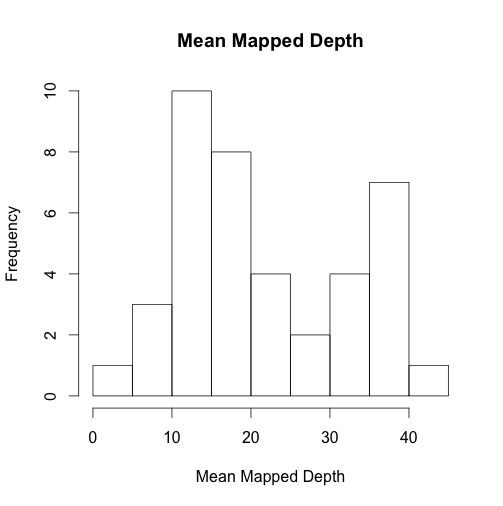
\includegraphics[width=0.8\textwidth]{depthBQ20MQ30.png}
  \caption{Mean mapped depth of sequenced used in analysis}
  \label{fig:depth}
\end{figure}

\begin{figure}[b]
\centering
   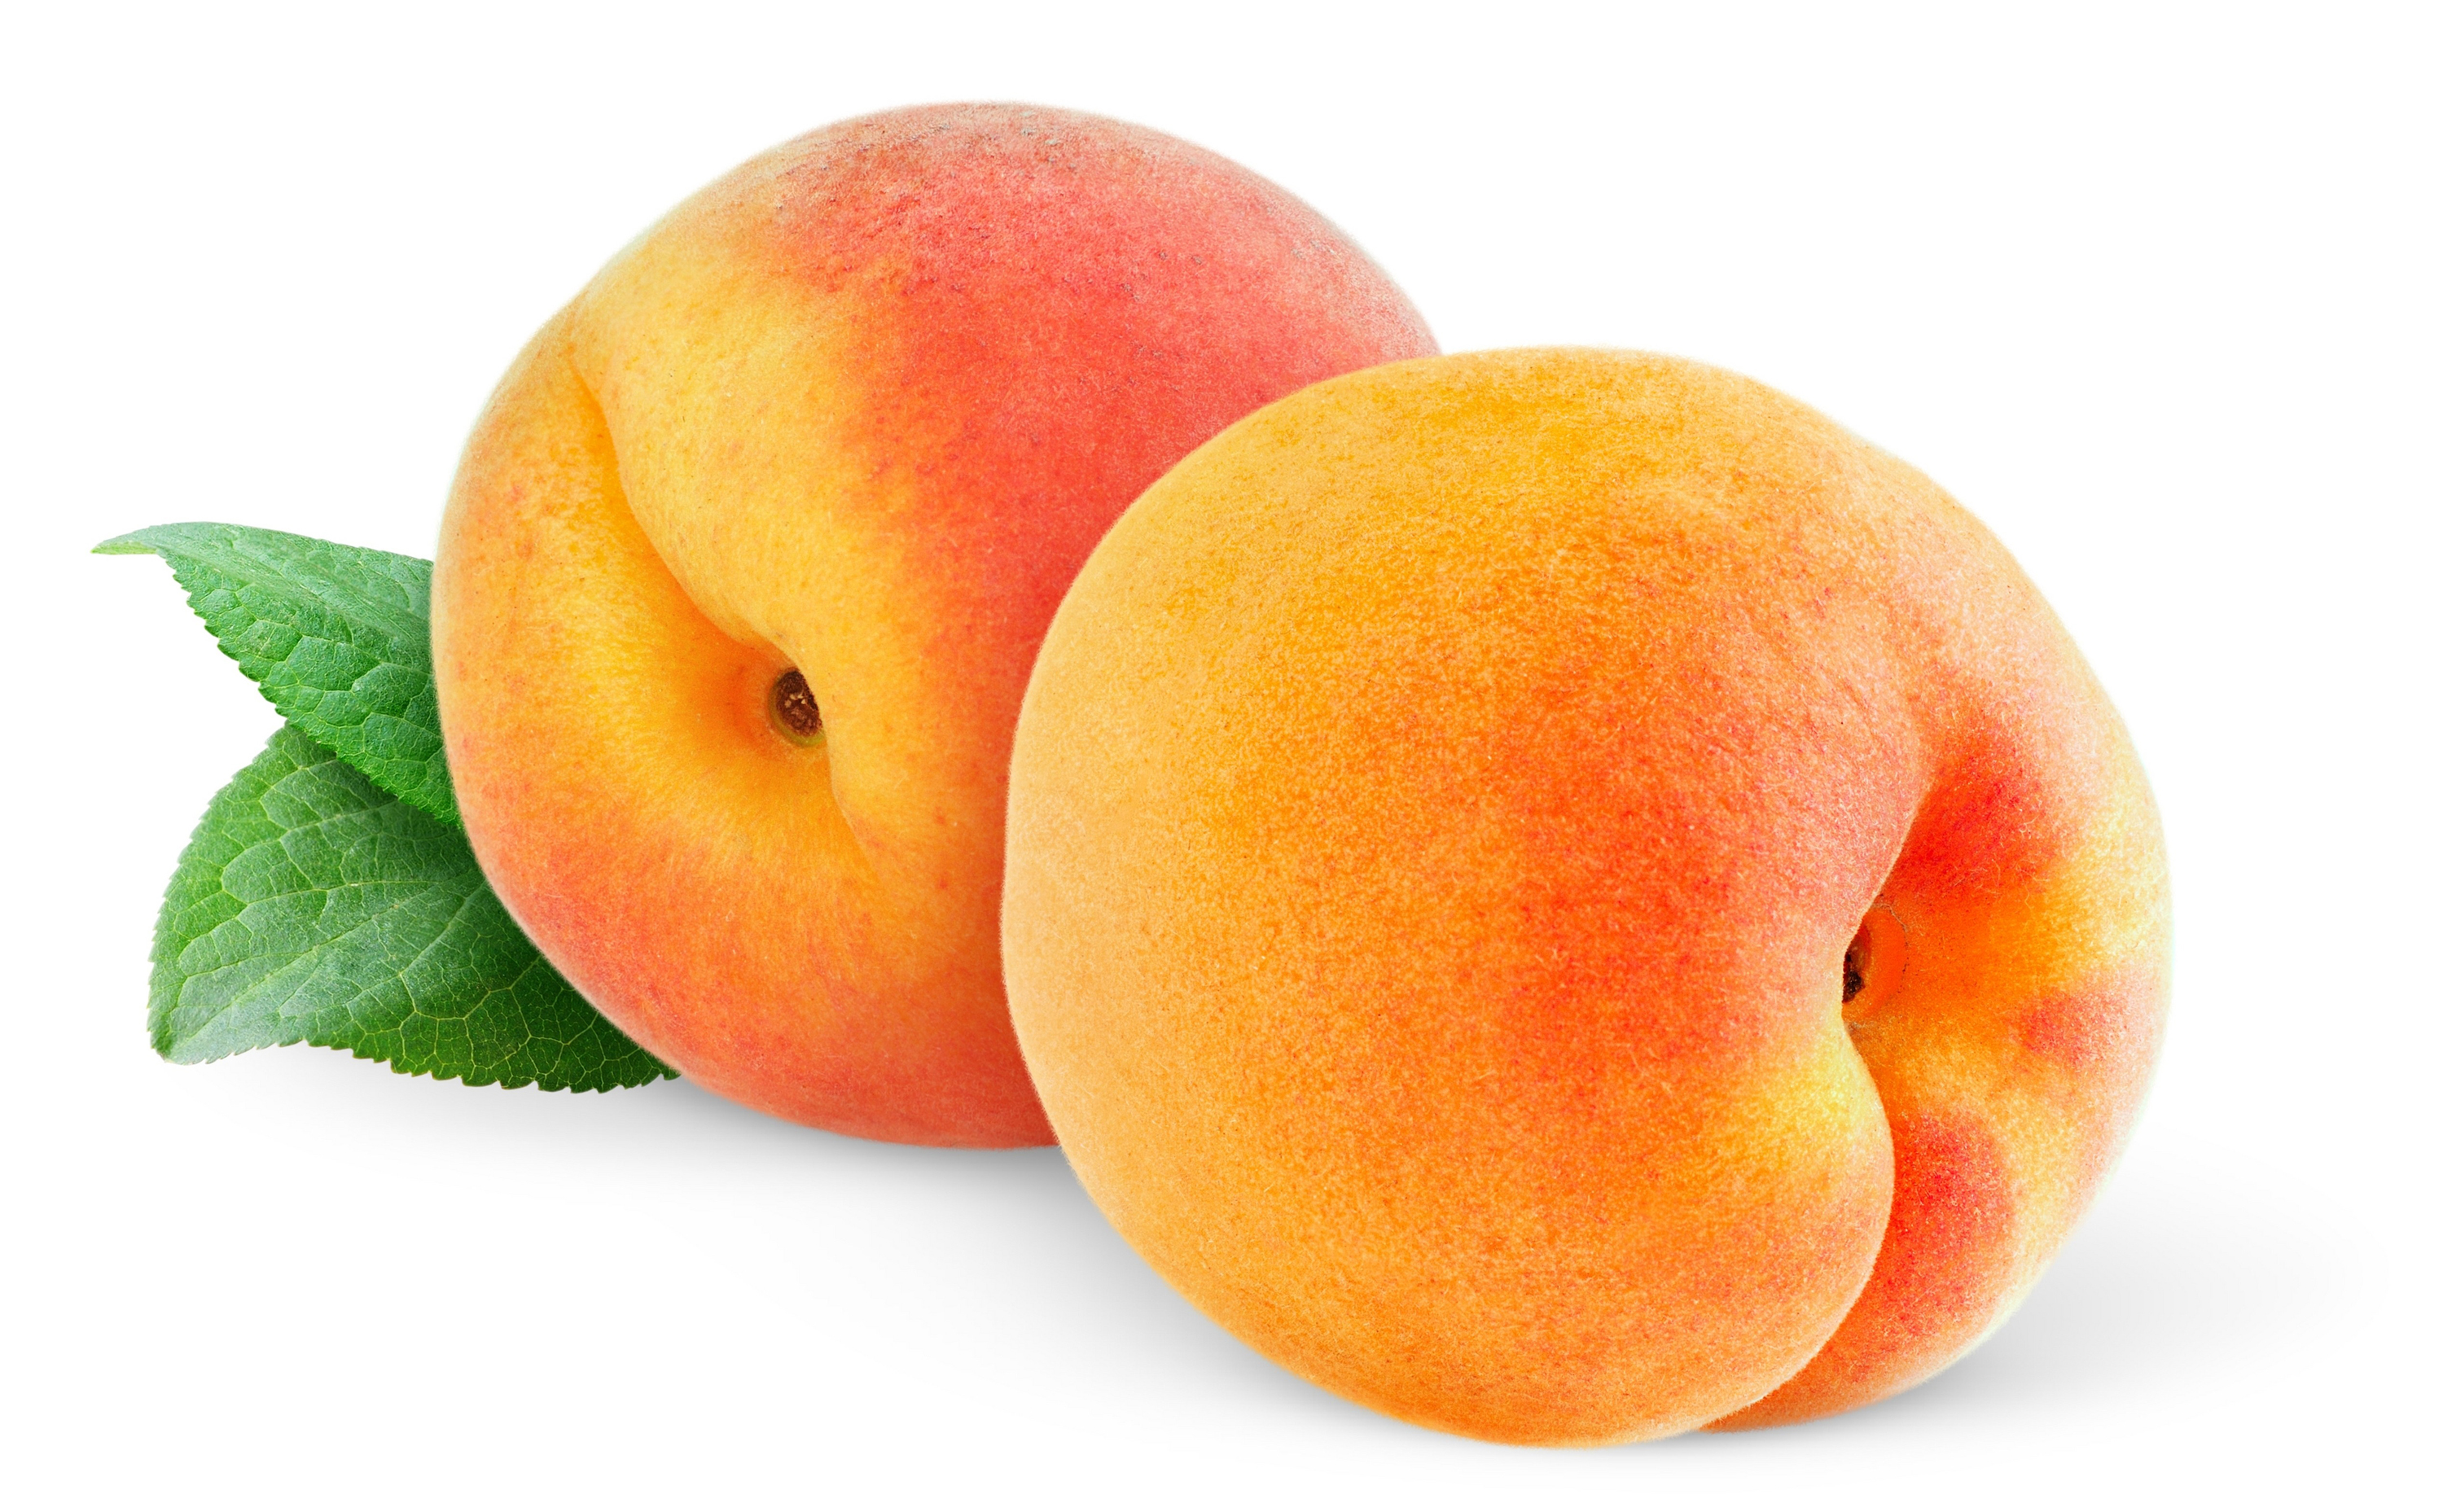
\includegraphics[width=0.8\textwidth]{peachzdfgad.jpg}
  \caption{Delicious peaches although the really new stuff in the paper will be about almonds}
  \label{fig:peach}
\end{figure}
%
\pagebreak
\beginsupplement
\section*{Supplementary Data}
%somehow change table number also maker table width match full width of text
\begin{center}
\begin{longtable}{lllll}
\caption[P. dulcis, P. persica and related species used in analysis.]{P. dulcis, P. persica and related species used in analysis.} \label{my-label} \\
\hline \hline \multicolumn{1}{l}{\textbf{Sample ID}} &
\multicolumn{1}{l}{\textbf{Accession and/or Cultivar}} &
\multicolumn{1}{l}{\textbf{Origin}} &
\multicolumn{1}{l}{\textbf{Source}}  &
\multicolumn{1}{l}{\textbf{Reference}} \\ \hline 
\endfirsthead

\multicolumn{5}{r}{{\bfseries \tablename\ \thetable{} -- continued from previous page}} \\
\hline \multicolumn{1}{l}{\textbf{Sample ID}} &
\multicolumn{1}{l}{\textbf{Accession and/or Cultivar}} &
\multicolumn{1}{l}{\textbf{Origin}} &
\multicolumn{1}{l}{\textbf{Source}} &
\multicolumn{1}{}{\textbf{Reference}} \\ \hline 
\endhead

\hline \multicolumn{5}{r}{{Continued on next page}} \\ \hline
\endfoot

\hline \hline
\endlastfoot

                 \multicolumn{5}{l}{\emph{P. dulcis}}  \\
%		 PD01 &DPRU 2578.2 & &NCGR &this study\\
		%Almond Board resequencing (BGI)
		% Not included because it appears to be possible F1 of peach x almond (or reverse)
                 PD02 &‘Tardy Nonpareil’ &USA &UCD &1\\
		%Almond Board resequencing (BGI)
                 PD03 &DPRU 1791.3, BE-1609 &Turkey &NCGR &1\\
		%Jastro resequencing (performed at UC Berkeley)
                 PD04 &DPRU 2374.12 &Iran &NCGR &1\\
		%Jastro resequencing (performed at UC Berkeley)
                 PD05 &DPRU 1456.4, Badam &Pakistan &NCGR &1\\
		%Jastro resequencing (performed at UC Berkeley)
                 PD06 &DPRU 2301, Tuono &Italy &NCGR &1\\
		%Jastro resequencing (performed at UC Berkeley)
                 PD07 &DPRU 1462.2 &Pakistan &NCGR &1\\
		%Jastro resequencing (performed at UC Berkeley)
                 PD08 &DPRU 1207.2 &Uzbekistan &NCGR &1\\
		%Jastro resequencing (performed at UC Berkeley)
                 PD09 &DPRU 2331.9 &China &NCGR &1\\
		%Jastro resequencing (performed at UC Berkeley)
                 PD10 &DPRU 0210, Languedoc &France &NCGR &1\\ %Jastro resequencing (performed at UC Berkeley)
                 PD11 &S3067 &Spain &SRR765861 &2\\
		% resequenced at WSU by Amit Dhingra
                 PD12 &D05-187 &Spain &SRR765850 &2\\
		% resequenced at WSU by Amit Dhingra
                 PD13 &Lauranne &Spain &SRR765838 &2\\
		% resequenced at WSU by Amit Dhingra
                 PD14 &Ramillete &Spain &SRR765679 &2\\
		% resequenced at WSU by Amit Dhingra
                 PD15 &Nonpareil & USA&RosBREED &5\\
                 \\
                 \multicolumn{5}{l}{\emph{P. persica}}  \\ % format italics
                 %PP01 &Lovell &USA &SRR502985 &3\\
                 % resequenced doubled haploid
                 PP02 &Yumyeong &Korea &SRR502994 &3\\
                 PP03 &Shenzhou Mitao&N China &
		\multirow{2}{1cm}{SRR502993, SRR502992} &3\\
                 %honey peach
                 \\
                 PP04 &Sahua Hong Pantao &S China &
		\multirow{2}{1cm}{SRR502991, SRR502990} &3\\
                 %flat peach
                 \\
                 PP05 &Quetta &Pakistan &
		\multirow{2}{1cm}{SRR502989, SRR502987} &3\\
                 \\
                 PP06 &Oro A &Brazil &SRR502986 &3\\
		%
                 PP07 &IF7310828 &Italy &
		\multirow{2}{1cm}{SRR503001, SRR503000} &3\\
                 \\
                 PP08 &GF305 &France &SRR502983 &3\\
                 %
		 PP09 &F$_{1}$ Contender $\times$ Ambra &Italy &SRR502997 &3\\
                 % peach x nectarine both P. persica
                 PP10 &Earligold &USA &
		\multirow{2}{1cm}{SRR502996, SRR502995} &3\\
                %  
		\\
                 PP11 &Bolero &Italy &SRR501836 &3\\
		 %
                 %PP12 &F8,1-42 &USA &SRR068361 &4\\
                 % Nonpareil almond in pedigree
		 % use for introgression investigation
		 PP13 &Georgia Belle &USA &SRR068359 &4\\
		 %
                 PP14 &Dr. Davis &USA &SRR068360 &4\\
		 % 
                 PP15 &Lovell &USA &UCD &1\\
                 % originally a canning variety selected ~1882
		 % currently used as rootstock and/or control for disease screening
                 % FPS, ABC
                 % duplicate cultivar, BGI sequenced at higher depth
                 PP16 &DPRU 1190, Admiral Dewey&USA &RosBREED &5\\
                 %aka PI 673525; introduced 1899
                 PP17 &Babcock &USA &RosBREED &5\\
                 %introduced 1897
                 PP18 &Bolinha &Brazil &RosBREED &5\\
		 % released 1985
		 % parentage: prob OP Aldrighi (Raseira et al. 1992; http://hortsci.ashspublications.org/content/27/11/1154.full.pdf)
		 %considered resistant to brown rot (Monilinia fructicola); low chill
                 PP19 &DPRU 2142, Carman &USA &RosBREED &5\\
		 %Planted 1889 from OP seed (unknown variety) by J. W. Stubenrauch, Mexia, TX
		 % data entry error listed as Carmen in GRIN; PI book has Carman
		 % http://sun.ars-grin.gov:8080/npgs_public/prodweb.pdf0?in_vol=33&in_suffix=&in_page=052
                 % PI 673586; cultivar original PI 34673 assigned 1912
                 PP20 &Chinese Cling&China &RosBREED &5\\
                 %introduced 1850; founder several cultivars
                 PP21 &Diamante&Brazil &RosBREED &5\\
                 %predominant canning cultivar in Brazil per Okie (year & pub TBD)
                 PP22 &Dixon&USA &RosBREED &5\\
		% Introduced in 1956
		% http://www.google.com/patents/USPP13911
		% early cling peach
                 %PP23 &Dr. Davis& &RosBREED &5\\
                 % duplicate cultivar
                 PP24 &DPRU 0589, Early Crawford &USA &RosBREED &5\\
                 %introduced before 1832
                 PP25 &Elberta&USA &RosBREED &5\\
                 %introduced ~1889; OP sdlg of 'Chinese Cling’
                 PP26 &Florida Prince P138&USA &RosBREED &5\\
                 %low chill cultivar; introduced in 2009
                 %PP27 &Georgia Bell&USA &RosBREED &5\\
                 %(aka ‘Georgia Belle’ and ‘Belle of Georgia’
		% introduced ~1875; OP sdlg of Chinese Cling)
                 %duplicate cultivar
                 PP28 &JH Hale&USA &RosBREED &5\\
                 %male sterile; introduced 1912
                 %PP29 &Lovell &USA &RosBREED &5\\
                 PP30 &Mayflower&USA &RosBREED &5\\
                 %introduced 1909
                 PP31 &Nemaguard &USA &RosBREED &5\\
                 %rootstock; rumored to have P. davidiana in pedigree
                 PP32 &O'Henry &USA &RosBREED &5\\
                 %plant patent 2.964 1/27/1970; OP sdlg Merrill Bonanza; discovered 1960
                 PP33 &Okinawa &Japan &RosBREED &5\\
		% Sharpe 1957
		% http://fshs.org/proceedings-o/1957-vol-70/320-322%20%28SHARPE%29.pdf
		% from 1953 seed lot, different seedlings
		%unsure if only one of these is what is now called 'Okinawa'
		% has nematode resistance
		% used in hybrid combination with Harrow's Blood (F2s) as rootstock
                 PP34 &Oldmixon Free &USA &RosBREED &5\\
                 % introduced 1832
                 PP35 &Rio Oso Gem &USA &RosBREED &5\\
                 % introduced 1933
		% developed in Rio Oso, California, Sierra Nevada foothills
		% https://www.slowfoodusa.org/ark-item/rio-oso-gem-peach
                 PP36 &DPRU 2179, Slappey &USA &RosBREED &5\\
                 %aka ‘Slappy’ in GRIN; introduced 1903
                 PP37 &DPRU 0941, St. John Yellow &USA &RosBREED &5\\
                 %introduced 1860s
                 %some variety history at http://gapeaches.org/about-us/father-of-the-ga-peach-industry/
		\\
                 \multicolumn{5}{l}{Other \emph{Prunus} species}  \\
                 %Almond Board resequencing (performed at BGI)
                 PF01 &\emph{P. fenzliana} &? &UCD &1\\
                 %UCD,ABC
                 PG01 &\emph{P. ferganensis} &Fergana Valley &
		\multirow{2}{1cm}{SRR502999, SRR502998} &3\\
                 \\
                 PC01 &\emph{P. cerasifera} DPRU 0579, Myrobalan &USA &NCGR &1\\ \hline
                 %outgroup
                 %NCBI SRA
               %note that the SRR IDs are from NCBI SRA
               %GDR/RosBREED (ftp://ftp.bioinfo.wsu.edu/species/Prunus_persica/RosBREED_Illumina/)

\end{longtable}
\end{center}
$^{1}$ this study\\
$^{2}$ \citealt{koepke2013comparative}?\\
$^{3}$ \citealt{verde2013high}\\
$^{4}$ \citealt{ahmad2011whole}\\
$^{5}$ \url{ftp://ftp.bioinfo.wsu.edu/www.rosbreed.org/resequencing/Prunus_persica/}\\
\endsupplement
\end{document}
